\documentclass{article}
\title{The mixup data}
\usepackage{graphicx}
\usepackage{Statweave}
\begin{document}
\maketitle
The data:
\begin{verbatim}
a 1 2
a 1 5
a 2 3
a 1 4
b 5 7
b 4 4
b 7 5
b 6 5
c 6 6
c 7 4
c 4 7
c 4 5
\end{verbatim}
The SAS code and output:
\begin{Winput}
data mix;
    infile "mixup.dat";
    input group $ x y;

proc gplot;
    plot y*x=group;
\end{Winput}
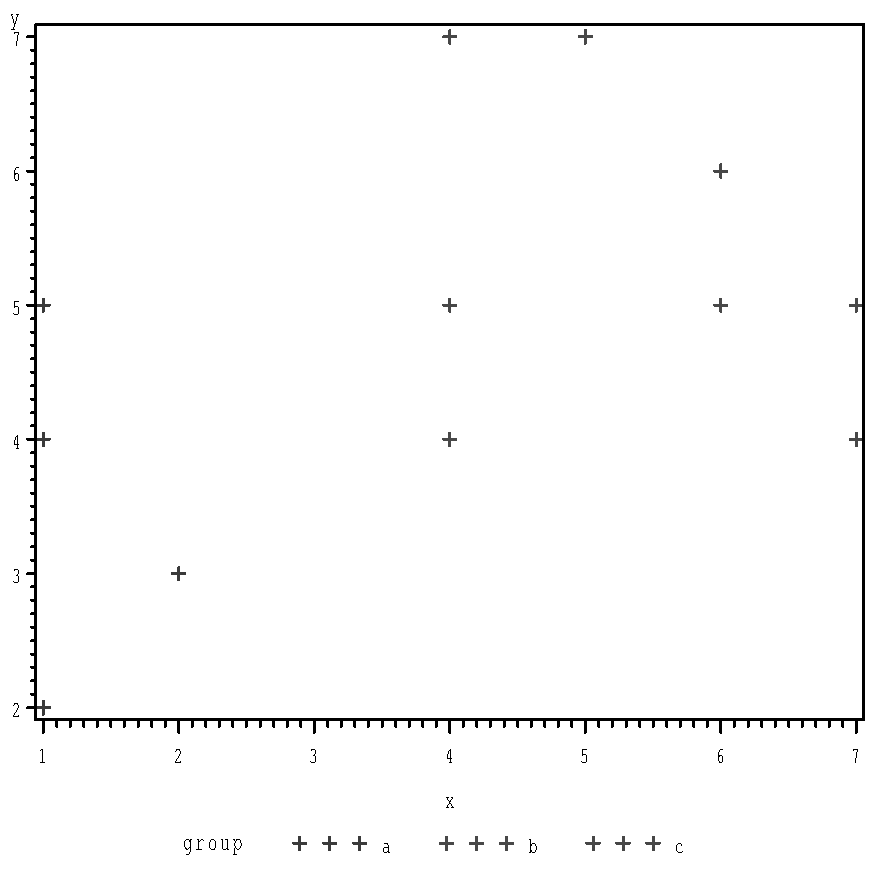
\includegraphics[]{mixup-1-SAS-fig.pdf}
    
\begin{Winput}
proc discrim can list out=xx;
    class group;
    var x y;
    
proc print;

proc gplot;
    plot Can1 * Can2 = group;

run;
\end{Winput}
\begin{Woutput}
The DISCRIM Procedure
Total Sample Size       12          DF Total                11
Variables                2          DF Within Classes        9
Classes                  3          DF Between Classes       2

Number of Observations Read             12
Number of Observations Used             12

                        Class Level Information
         Variable                                                  Prior
group    Name        Frequency       Weight    Proportion    Probability
a        a                   4       4.0000      0.333333       0.333333
b        b                   4       4.0000      0.333333       0.333333
c        c                   4       4.0000      0.333333       0.333333

Pooled Covariance Matrix Information
               Natural Log of the
 Covariance    Determinant of the
Matrix Rank     Covariance Matrix
          2               0.75377

The DISCRIM Procedure
Pairwise Generalized Squared Distances Between Groups
 2         _   _       -1  _   _
D (i|j) = (X - X )' COV   (X - X )
            i   j           i   j

     Generalized Squared Distance to group
From
group              a             b             c
a                  0      18.65441      17.88235
b           18.65441             0       0.06618
c           17.88235       0.06618             0

The DISCRIM Procedure
Canonical Discriminant Analysis
                           Adjusted    Approximate        Squared
           Canonical      Canonical       Standard      Canonical
         Correlation    Correlation          Error    Correlation
       1    0.918688       0.909728       0.047039       0.843988
       2    0.112797        .             0.297675       0.012723
                                                      Test of H0: The canonical correlations in the
                   Eigenvalues of Inv(E)*H               current row and all that follow are zero
                     = CanRsq/(1-CanRsq)
                                                     Likelihood Approximate
         Eigenvalue Difference Proportion Cumulative      Ratio     F Value Num DF Den DF Pr > F
       1     5.4098     5.3969     0.9976     0.9976 0.15402685        6.19      4     16 0.0033
       2     0.0129                0.0024     1.0000 0.98727677        0.12      1      9 0.7412

The DISCRIM Procedure
Canonical Discriminant Analysis
         Total Canonical Structure
Variable              Can1              Can2
x                 0.963543         -0.267552
y                 0.675253          0.737586

        Between Canonical Structure
Variable              Can1              Can2
x                 0.999419         -0.034073
y                 0.991126          0.132925

     Pooled Within Canonical Structure
Variable              Can1              Can2
x                 0.819802         -0.572647
y                 0.341984          0.939706

The DISCRIM Procedure
Canonical Discriminant Analysis
Total-Sample Standardized Canonical Coefficients
Variable              Can1              Can2
x              1.894981189      -0.689633325
y              0.687386181       0.984062813

Pooled Within-Class Standardized Canonical Coefficients
Variable              Can1              Can2
x             0.9725702950      -.3539438228
y             0.5926742015      0.8484730398

         Raw Canonical Coefficients
Variable              Can1              Can2
x             0.8252532609      -.3003312927
y             0.4629576531      0.6627706863

   Class Means on Canonical Variables
group              Can1              Can2
a          -2.848143534      -0.002552303
b           1.469358718      -0.119111596
c           1.378784816       0.121663899

The DISCRIM Procedure
Linear Discriminant Function
               _     -1 _                              -1 _
Constant = -.5 X' COV   X      Coefficient Vector = COV   X
                j        j                                 j

      Linear Discriminant Function for group
Variable             a             b             c
Constant      -5.40645     -25.95670     -25.79861
x              1.60458       5.20261       5.05556
y              2.51634       4.43791       4.55556

The DISCRIM Procedure
Classification Results for Calibration Data: WORK.MIX
Resubstitution Results using Linear Discriminant Function
Generalized Squared Distance Function
 2         _       -1   _
D (X) = (X-X )' COV  (X-X )
 j          j            j
Posterior Probability of Membership in Each group
                   2                    2
Pr(j|X) = exp(-.5 D (X)) / SUM exp(-.5 D (X))
                   j        k           k

      Posterior Probability of Membership in group
       From      Classified
Obs    group     into group         a         b         c
  1    a         a             1.0000    0.0000    0.0000
  2    a         a             0.9982    0.0006    0.0012
  3    a         a             0.9989    0.0005    0.0006
  4    a         a             0.9998    0.0001    0.0002
  5    b         c        *    0.0000    0.4387    0.5613
  6    b         c        *    0.0961    0.4428    0.4611
  7    b         b             0.0000    0.5703    0.4297
  8    b         b             0.0000    0.5339    0.4660
  9    c         b        *    0.0000    0.5046    0.4954
 10    c         b        *    0.0000    0.5989    0.4011
 11    c         c             0.0003    0.4028    0.5969
 12    c         c             0.0144    0.4539    0.5317
* Misclassified observation

The DISCRIM Procedure
Classification Summary for Calibration Data: WORK.MIX
Resubstitution Summary using Linear Discriminant Function
Generalized Squared Distance Function
 2         _       -1   _
D (X) = (X-X )' COV  (X-X )
 j          j            j
Posterior Probability of Membership in Each group
                   2                    2
Pr(j|X) = exp(-.5 D (X)) / SUM exp(-.5 D (X))
                   j        k           k

 Number of Observations and Percent Classified into group
From
group             a            b            c        Total
a                 4            0            0            4
             100.00         0.00         0.00       100.00
b                 0            2            2            4
               0.00        50.00        50.00       100.00
c                 0            2            2            4
               0.00        50.00        50.00       100.00
Total             4            4            4           12
              33.33        33.33        33.33       100.00
Priors      0.33333      0.33333      0.33333

              Error Count Estimates for group
                       a           b           c       Total
Rate              0.0000      0.5000      0.5000      0.3333
Priors            0.3333      0.3333      0.3333

Obs    group    x    y      Can1        Can2         a          b          c       _INTO_
  1      a      1    2    -3.74889    -0.92163    1.00000    0.00000    0.00000      a
  2      a      1    5    -2.36002     1.06669    0.99818    0.00065    0.00117      a
  3      a      2    3    -2.46068    -0.55919    0.99887    0.00051    0.00063      a
  4      a      1    4    -2.82298     0.40392    0.99975    0.00009    0.00015      a
  5      b      5    7     1.86691     1.19090    0.00001    0.43873    0.56127      c
  6      b      4    4    -0.34722    -0.49708    0.09606    0.44283    0.46111      c
  7      b      7    5     2.59150    -0.73530    0.00000    0.57030    0.42970      b
  8      b      6    5     1.76625    -0.43497    0.00001    0.53395    0.46604      b
  9      c      6    6     2.22920     0.22780    0.00000    0.50459    0.49540      b
 10      c      7    4     2.12854    -1.39807    0.00000    0.59886    0.40113      b
 11      c      4    7     1.04165     1.49123    0.00027    0.40279    0.59693      c
 12      c      4    5     0.11574     0.16569    0.01441    0.45392    0.53166      c
\end{Woutput}
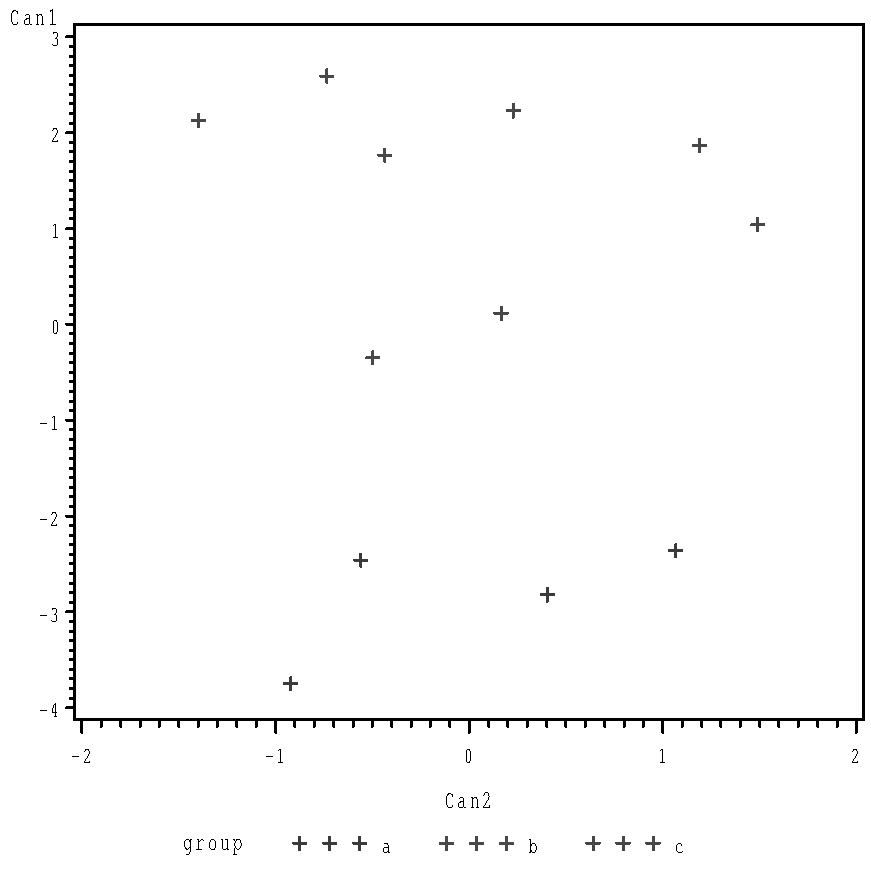
\includegraphics[]{mixup-2-SAS-fig.pdf}
\end{document}
